% \newpage

%---------------------------------------------------------------------------------
% Approach
%---------------------------------------------------------------------------------

\section{Approach}

\subsection{Simplifying the Model}

\quad Either football team has 11 players. It can be difficult to hardcode all these "robots", or players, so we seek to make a few simplifications. We first reduce our number of players, then restrict the particular play they're running, reduce the dimensions, and re-frame things to focus on Quarterback safety.

\subsubsection{Categorical Players}

\quad We will reduce our model to a total of 6 robots, or "player categories". We will have a Quarterback, Offensive Lineman, Defensive Lineman, Wide Receiver, and Linebacker. The Quarterback still is the same as in normal football, since there is one Quarterback on the offensive team. For the linemen (OL and DL), we will leverage the ideas from our related works section and view the various linemen on a football team as a "collective". Namely, there will be one robot who symbolizes the collective of the Offensive Line, and one for the Defensive Line. In real football, these linemen are in a relatively close position performing very similar actions, so viewing them as a collective will suffice for our model. \\

Finally, for the Wide Receiver and Linebacker, we will only consider one these "pairings". In real football, there will be a few different Wide Receivers to pass to, given the Quarterback's various options to make. By reducing it to one "pairing", we limit the Quarterback's possible options. It follows that if the Quarterback is able to safely pass with just one option, he only become "safer" with more options to pass to.

\subsubsection{Hail Mary}

\quad There are various plays in football which involve certain players running certain routes and such. This can lead to some undesired complexity, so for our model, we will pick a simple football play known as “Hail Mary.” We see that there are 5 Wide Receivers (WR), each with a forward arrow representing the path they will follow. Their goal is to run forward and catch the ball if it is thrown to them while avoiding contact from the Linebacker (LB). The dots with a seemingly inverted-T shaped root to them and are aggregated in the center represent our 5 Offensive Linemen (OL), whose goal is to protect the Quarterback (QB) from the Defensive Line (DL, not in picture). Finally, the last dot towards the bottom that is seemingly being protected, is the QB.\\

Since we have simplified our number of players as described above, we will not have these Wide Receivers in our model. The way we use a Hail Mary plan is to hard-code a route for our Wide Receiver to travel along. In a Hail Mary play, he will only move forward, so this simplifies the Ordinary Differential Equation we will use to model his movement. Hard-coding the WR's path like this is still accurate to real life football since the Quarterback decides the play that is being run. In a sense, the QB decides the ODE's of the offensive players. \\

\begin{figure}[htp]
    \centering
    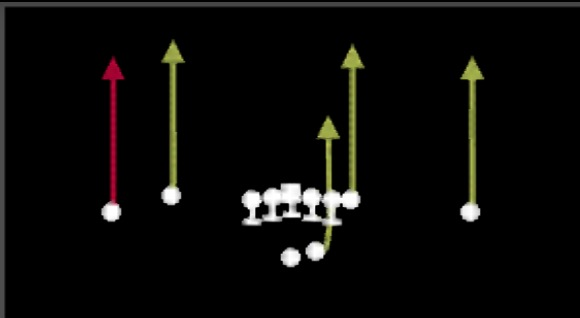
\includegraphics[width=7cm]{figure/hailMary.png}
    \caption{A depiction of a Hail Mary Pass in video game NFL Mobile.}
\end{figure}

\subsubsection{One Dimension}

\quad While football is a two-dimensional game, we are able to simplify the model into one dimension: the y-dimension. This simplification is due to the Hail Mary play relying on straight line movement up the field. This model is easily scalable to two dimensions, as the Quarterback only gets safer with more passing and maneuvering options. Furthermore, you can see that the Hail Mary play is roughly symmetric, so modelling it in a single y-dimension, would serve as an important stepping stone to modelling multiple instances of Wide Receivers. The proof would be very similar as the one-dimension case, just along different points of the x-axis.

\subsubsection{The Equivalence of Openness and Passing}

\quad One assumption that we will make is that openness is equivalent to passing. The main problem we seek to discuss is whether our Quarterback safely pass the ball? As such, we will assume that, when presented with the opportunity, our Quarterback will pass the ball to the Wide Receiver as soon as he becomes open. This means that our system has successfully protected the Quarterback for the necessary duration. As such, we will not worry about the physical act of passing for our model since we are focusing on the safety of the Quarterback. Though it is a bit unrealistic to say that the Quarterback can instantaneously pass the ball to the Wide Receiver, we will use this assumption to simplify our model and put a larger focus on Quarterback safety. 

\subsection{Realistic Magnitudes}

\quad Some things we will need to keep in mind for our model are realistic conditions. We are able to set these values and not leave them up to further generality because football is "defined" to have some of these constraints. The first will be the dimensions of the football field, and the speeds of the players. 

\subsubsection{Player Speeds}

\quad We gathered data from the NFL Combine (an event where prospective football players participate in various events to demonstrate their physical abilities) to determine appropriate speeds for our various players [1]. A 40 yard dash time is how long it takes a player to run 120 feet at a full sprint. Note that Quarterbacks usually move slowly since they need to be in a stable position to throw far distances. We model this by setting the QB's speed to the average pace at which a human walks. To get their speed in feet per second we do $120 \div dash$. Since we have this notion of a categorical player, we can reduce each player to their positions and find statistics per positions (Table 1). 

\newpage

\begin{table}[h]
    \centering
    \begin{tabular}{ |c|c|c| } 
     \hline
     \textbf{Position}\footnotemark & \textbf{40-yard Dash Time} & \textbf{Feet Per Second} \\ 
     \hline
     Quarterback & -- & 4.6 \\ 
     Wide Receiver & 4.48 & 26.79 \\ 
     Linebacker & 4.76 & 25.21 \\ 
     Defensive Lineman & 5.06 & 23.71 \\ 
     Offensive Lineman & 5.34 & 22.47 \\ 
     \hline
    \end{tabular}
    \caption{Times from the NFL Combine}
\end{table}


\footnotetext{Here we refer to specifically the Inside Linebacker. Defensive Lineman can also be called Defensive Tackles. finally, The Offensive Lineman is the average of the Offensive Guard and Tackle.}

\subsubsection{The Football Field}

\quad The football field’s dimensions are 160 feet by 300 feet. If we consider the football field to be on a coordinate plane, with the units being in feet, we will let the lower left corner be at the point (0, 0), the upper right corner be at (160, 300), and the center be at (80, 150). We will also consider the scenario where the Quarterback starts at this halfway point in our model (Figure 2).

\begin{figure}[htp]
    \centering
    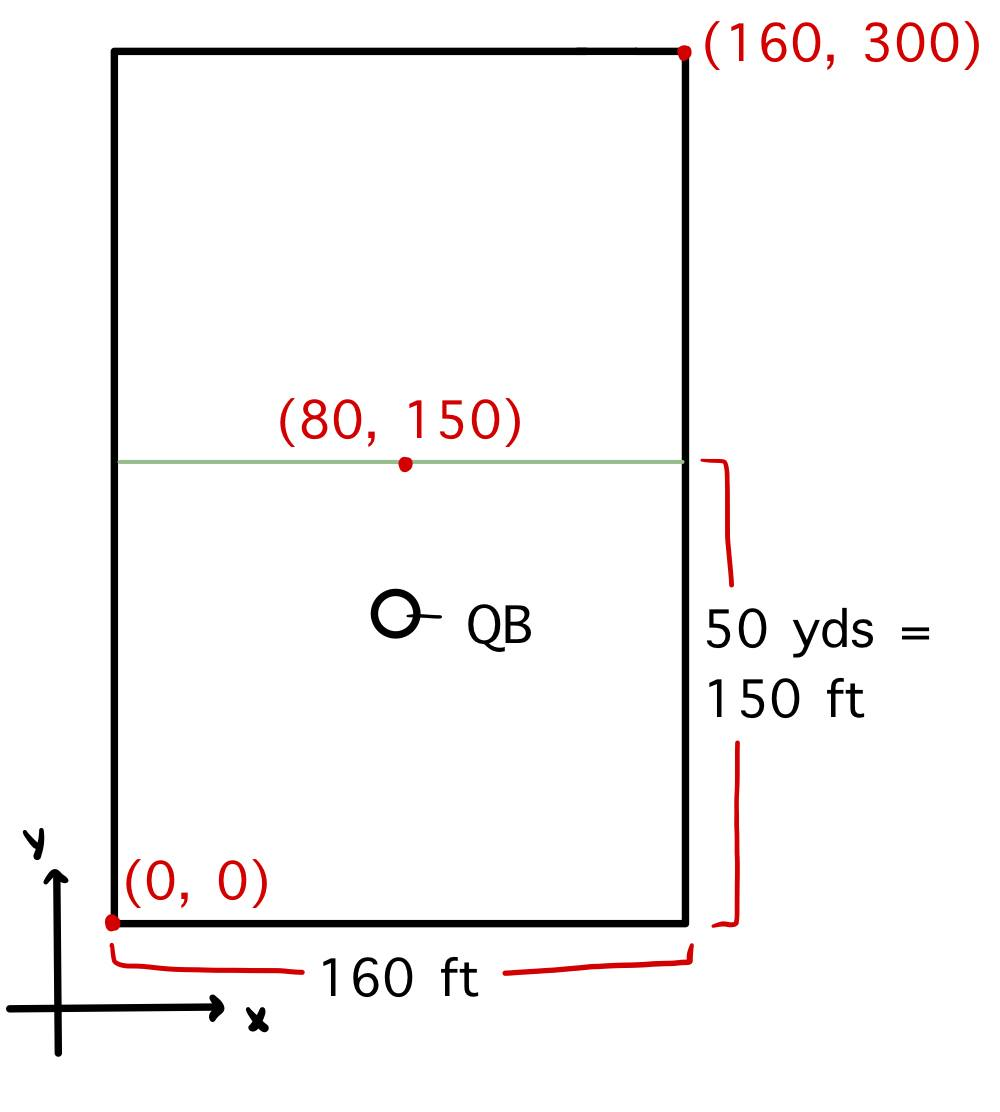
\includegraphics[width=5cm]{figure/1_dimensions.jpg}
    \caption{Geometrical dimensions of a NFL football field}
\end{figure}

\subsection{The Players}

\quad We will break the system down into its smaller subparts, by first examining how the Offensive and Defensive Lines work. To simplify the system, we will consider the Offensive Line and Defensive Line as their own single lines that move as a unit rather than individual players. In real football, the players might struggle to break past one another. For our model, we will simplify this by saying that the Defensive Line slowly approaches the Quarterback.

\subsubsection{Linemen Collision}
\quad  In football, there is no fixed rule as to where the Offensive and Defensive Lines need to start exactly. The only constraint is that the Offensive Line starts in front of the Quarterback on one side of the Line of Scrimmage and the Defensive Line starts on the other side of the Line of Scrimmage as visible in the visual. We will be viewing the football field from the perspective of the offense. \\

Note that the Offensive Line’s duty is to protect the Quarterback and the Defensive Line’s goal is to tackle the Quarterback before he throws the ball. Therefore the Defensive Line travels toward the Quarterback, which is the negative direction on the y-axis ($dy_D$). On the other hand, the Offensive Line travels away from the Quarterback, which means they travel in the positive direction on the y-axis ($dy_A$). To simplify the model, we consider that both of the lines travel with a constant velocity before they collide. We visualize the velocities and directions of the two lines in the following diagram (Figure 3). \\

\begin{figure}[htp]
    \raisebox{-0.08\height}{
    \hspace*{1.75cm}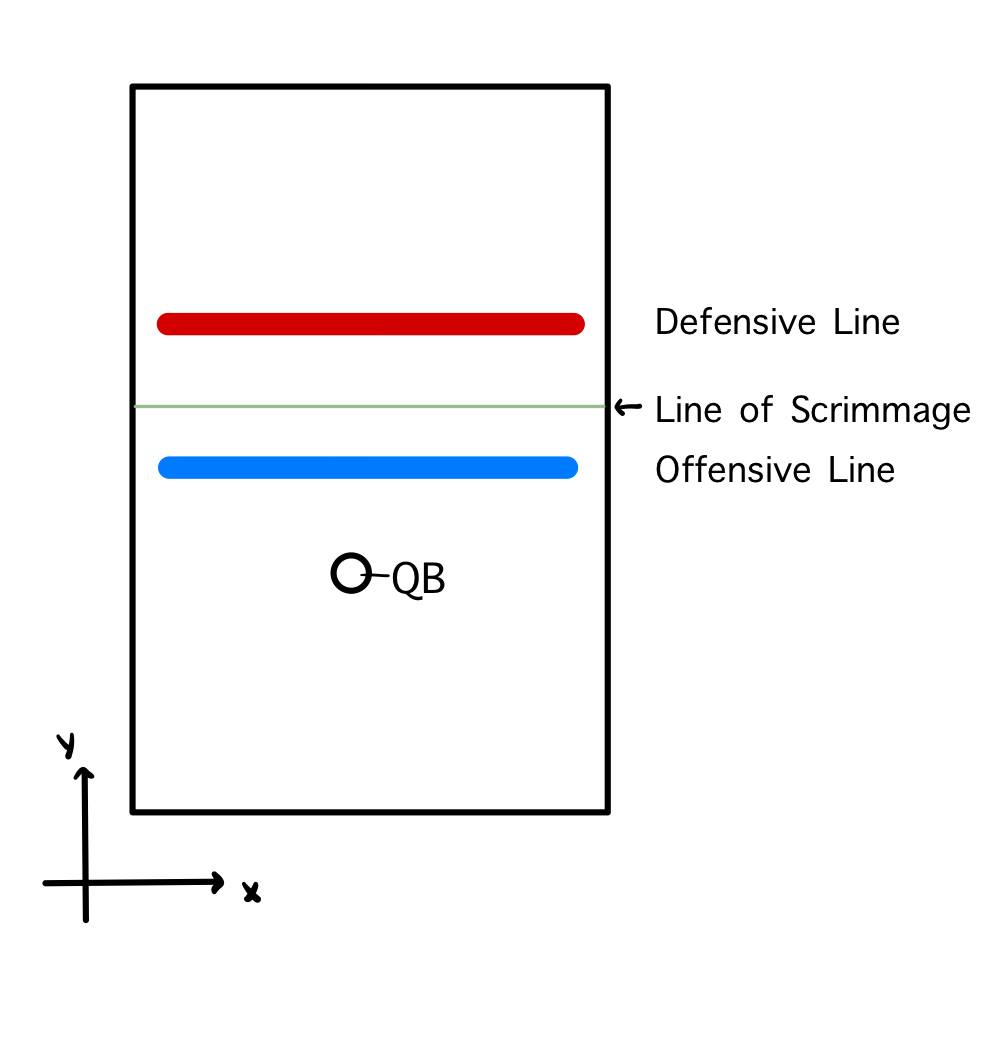
\includegraphics[width=6.62cm]{figure/2_line_layout.jpg}
    }
    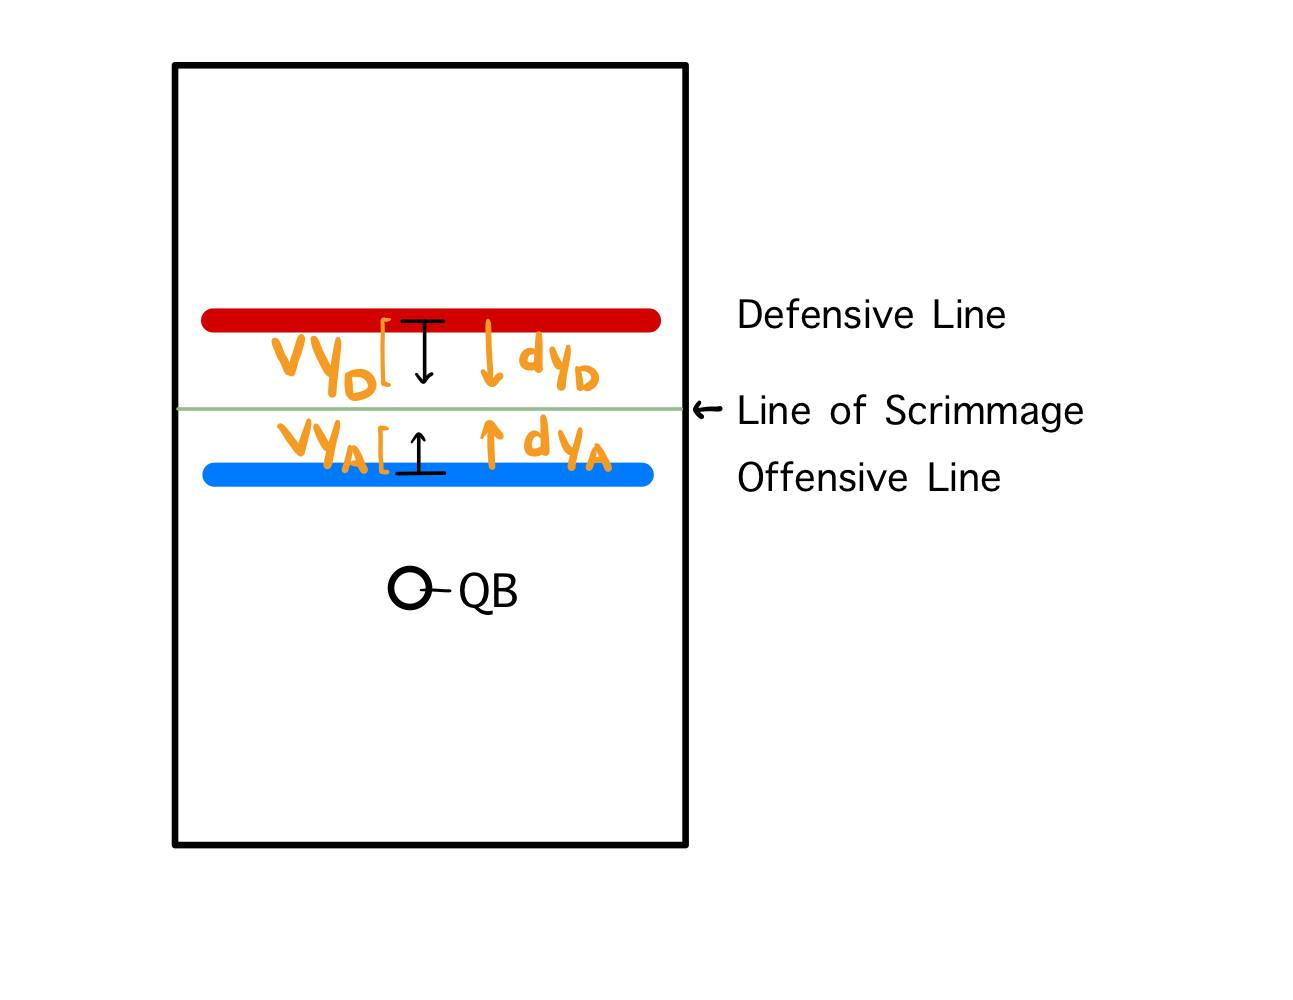
\includegraphics[width=7.8cm]{figure/3_line_velocities.jpg}
    \caption{Layout of Offensive and Defensive Lines}
\end{figure}

The Defensive Line, represented by the red line, is moving with speed $vy_D$ in the direction $dy_D$, and the Offensive Line (blue) is moving with speed $vy_A$ in direction $dy_A$. Note that $vy_D$ and $vy_A$ are the magnitudes of the lines' velocities, and are therefore non-negative. 

\newpage
 
At the start of the play, the two lines will charge towards each other. However, once the two lines collide, they will move as one unit with the velocity being the sum of their initial velocities; this models a perfectly inelastic collision. From \textbf{3.2 Realistic Magnitudes}, we see that Defensive Linemen are on average faster than Offensive Linemen; we model this by making the magnitude of the initial velocity of the Defensive Line greater than the magnitude of the velocity of the Offensive Line. Therefore, when the two lines collide, their velocities will counteract one another, effectively dampening the velocity of the Defensive line. \\

One might think of this as two people pushing against one another, but one eventually dominating the other in terms of force, thus pushing them back. Taking into account the force of the Offensive and Defensive lines, we see that they will travel with a velocity that has a magnitude equivalent to half of the difference between the magnitudes of the initial Defensive and Offensive Line’s velocities. If we consider that the masses of the Offensive and Defensive Lines are the same, we know that this abides with the Principle of Momentum Conservation because of the following equations. \\

Let $m_A$ and $m_D$ be the masses of the Offensive and Defensive lines respectively, where $m_A = m_D = m$. Let $vy_{Ai}$ and $dy_{Ai}$ be the initial velocity (magnitude) and direction of the Offensive Line, $vy_{Di}$ and $dy_{Di}$ be the initial velocity (magnitude) and direction of the Defensive Line, and $vy_f$ and $dy_f$ be the final velocity and direction of both lines together after the collision. By the conservation of momentum, we have:
% Len: I changed this slightly because things are showing up weird on Overleaf
\begin{align*}
m_A \cdot vy_{Ai} \cdot dy_{Ai} + m_D \cdot vy_{Di} \cdot dy_{Ai} &= m_A \cdot vy_f \cdot dy_f + m_D \cdot vy_f \cdot dy_f \\
m(vy_{Ai} \cdot dy_{Ai} + vy_{Di} \cdot dy_{Ai}) &= 2 \cdot m \cdot vy_f \cdot dy_f & (m = m_A = m_D) \\
m(vy_{Ai} - vy_{Di}) &= 2 \cdot m \cdot vy_f \cdot dy_f & (vy_{Ai} = 1, vy_{Di} = -1) \\
vy_{Ai} - vy_{Di} &= 2 \cdot vy_f \cdot dy_f & (\text{eliminate m}) \\
\frac{vy_{Ai} - vy_{Di}}{2} &= -vy_f
\end{align*}

Since $vyDi > vyAi$ (the Defensive Line is faster than the Offensive Line), we know that the left hand side has to be negative as $\frac{vyAi - vyDi}{2} < 0$. Therefore, $vyf \cdot dyf < 0$, and $vyf$ is a magnitude so it cannot be negative. Therefore, $dyf = -1$, and the direction is the same as the Defensive Line’s original direction. We have $\frac{vyAi - vyDi}{2} = -vyf$. The progression of movement is shown in Figure 4.

\newpage

\begin{figure}[htp]
    \centering
    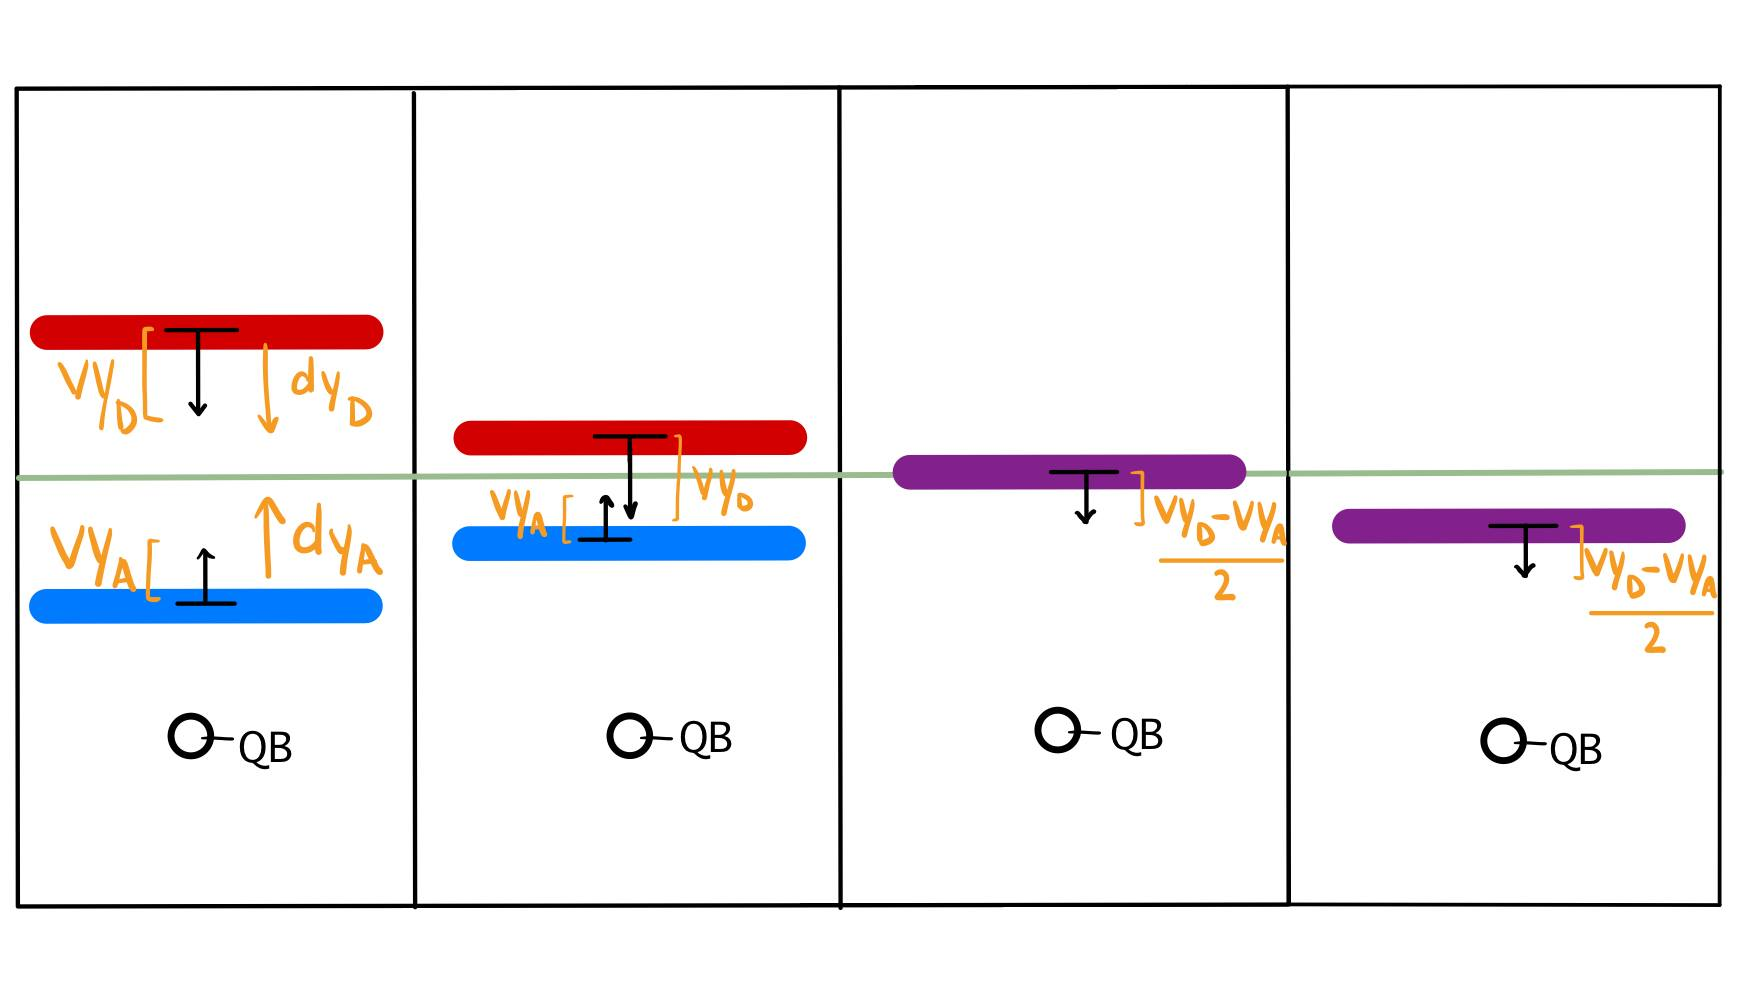
\includegraphics[width=12.5cm]{figure/4_line_evolution.jpg}
    \caption{Evolution of Offensive and Defensive Lines}
\end{figure}

\subsubsection{The Quarterback and Wide Receiver} % subsubsection of "the players"

\quad In football, the Quarterback is the player who passes the ball, so he has great control over how the offensive play is conducted. In order for us to successfully advance the ball up the field, it is essential for the Quarterback to remain safe enough to pass to the Wide Receivers. This requires that the Quarterback does not get tackled by the Defensive Line until he executes a pass. Recall from \textbf{1.3 Football Through The Lens of Hybrid Systems}, tackling is represented as the intersection of their y-coordinates. The winning strategy is dependent on two things: the Quarterback’s ability to both pass and stay away from the Defensive Line. \\

The Quarterback is able to avoid a collision with the Defensive Line by moving away from it. In this scenario, "away" would mean moving backwards from the Defensive Line. We also know that the Quarterback's speed is faster than the dampened Defensive Line speed, so his safety is ensured. Therefore, the only aspect remaining to ensure a successful run is whether the Wide Receiver can get open while all the players are still on the field. From \textbf{3.1.4 The Equivalence of Openness and Passing}, the Quarterback will pass as soon as the Wide Receiver is open. However, this notion of openness will be different in certain scenarios. We partition these scenarios into two defensive strategies, or their more colloquially known terms: "man" and "zone." 

\newpage

\subsubsection{Man Defense}

% Added by Len
\quad Recall that a "man-to-man", or "Man", defense is one where each Linebacker tightly guards a Wide Receiver. Since our model has been reduced to categorical players, this means that our Linebacker will start as close as he can to the Wide Receiver. As we will later formalize in \textbf{4.3 Preconditions}, this closest distance is the Line of Scrimmage. As such, our singular Linebacker will likely start where the Defensive Line starts as well. \\

% Added by Len
Since the Linebacker will be able to closely follow the Wide Receiver for the majority duration of his evolution (or his act of running forward), the Wide Receiver will only be open if he runs past the Linebacker. Within the context of our model, the Wide Receiver will become open if his y-coordinate is greater than the y-coordinate of the Linebacker. However, this relies on the speed of the Wide Receiver being greater. From earlier, we reasoned that the difference in speed between the two is rather small. This small difference thus requires a long distance or great amount of time in order for the Wide Receiver to "run past" the Linebacker. We will see later that this becomes very difficult to prove without using blatantly unrealistic preconditions.

\subsubsection{Zone Defense}

\quad Recall that a Zone Defense is one where the defensive players attempt to spread themselves out evenly throughout the field to cover all "zones", hence the name. For our model, this means that the Linebacker will start at some evenly spread distance behind the Defensive Line, which we will later formalize as roughly the halfway point between the Line of Scrimmage and the end of the field. The difference now is that there is a "healthy chunk" of distance between where the Wide Receiver and Linebacker starts. For our Quarterback, the decision to pass now suddenly flips. Instead of waiting for our Wide Receiver to run past the Linebacker like before, we now, we want to pass it before the Linebacker gets a chance to come down the field and tackle him. Notice that this means that the direction our Linebacker is traveling is flipped to the other direction, as is our notion of "openness". \\

We will show that this scenario is preferable for Quarterback safety. While in a Man defense scenario, we have a chance to pass it further and advance the ball down the field an even greater magnitude (in a sense having our controller be "more efficient"), this will be at the cost of compromising the safety of our Quarterback. In a Zone defense, while the distance which the ball moves forward may be less, our Quarterback will be provably safe. Through the lens of a hybrid system, this is much more desirable.
